\subsection{Detection Analysis}
\label{sub:evaluation-detection}



\paragraph{Exp\#1 (Similarity detection on plaintext chunks).}
We first justify that we can effectively find similar plaintext chunks by comparing content features. We consider multiple SYNChunk$(x, y)$, each of which includes 10\,K similar chunks (i.e., ground truth) modified from a base chunk (recall that $x$ defines the number of modified locations, and $y$ defines the number of modified bytes in each location, see \S\ref{sub:datasets}). We extract four content features for each plaintext chunk in SYNChunk$(x, y)$, and identify similar chunks if they share one to four identical features, respectively. We evaluate the fraction of the similar chunks that are successfully identified over all (similar) chunks in the ground truth.


\begin{figure}[t]
    \centering
    
\includegraphics[width=.3\textwidth]{pic/featurespy/plot/detection/syn/fixed_pq_legend.pdf}
    \vspace{5pt}\\
    \begin{tabular}{@{\ }c@{\ }c}
        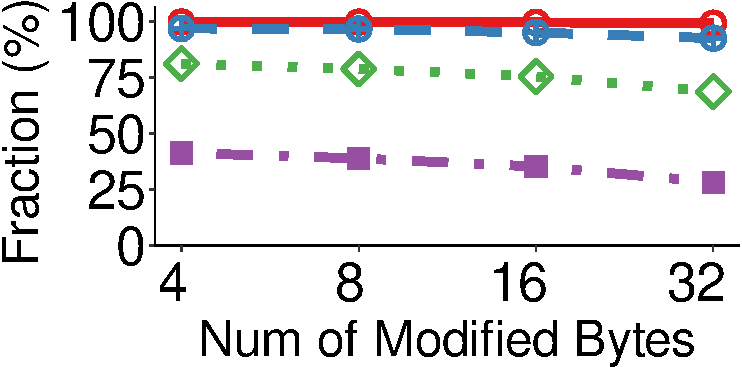
\includegraphics[width=0.23\textwidth]{pic/featurespy/plot/detection/syn/fixed_p_4.pdf} &
        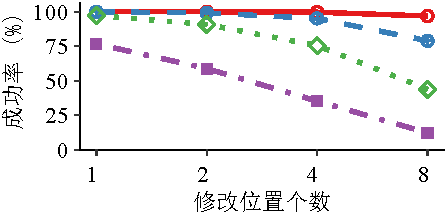
\includegraphics[width=0.23\textwidth]{pic/featurespy/plot/detection/syn/fixed_q_16.pdf}\\
        \mbox{\small (a) Fix $x=4$ and vary $y$}&
        \mbox{\small (b) Fix $y=16$ and vary $x$}\\
    \end{tabular}
    \vspace{-6pt}
    \caption{(Exp\#1) Similarity detection on plaintext chunks. We evaluate the fraction of the chunks that have some identical features over all similar chunks in each synthetic dataset SYNChunk$(x, y)$.}
    \vspace{-6pt}
    \label{fig:expDetectionSynSim}
\end{figure}


Figure~\ref{fig:expDetectionSynSim} shows the results when we use the SYNChunk$(x, y)$ that has a fixed $x$ = 4 and a varying $y$ (Figure~\ref{fig:expDetectionSynSim}(a)), as well as that has a fixed $y$ = 16 and a varying $x$ (Figure~\ref{fig:expDetectionSynSim}(b)). In general, the fraction of identified similar chunks degrades with $x$ and $y$, since significant modifications are likely to modify the content features of chunks. Specifically, the fraction is more affected by $x$ (than $y$), since increasing $x$ will change the Rabin fingerprints of a larger number of sliding windows (\S\ref{sub:basic}). On the other hand, we can effectively detect a large fraction (e.g., at least 78.9\%) of similar chunks by examining if they share one or two identical features.



\paragraph{Exp\#2 (Similarity detection on ciphertext chunks).}
We extend Exp\#1 to study the similarity detection of \sysnameF based on ciphertext chunks. We apply our design techniques and study the effectiveness of similarity preservation after the corresponding operations. Specifically, we perform feature key generation (via the proposed instances in \S\ref{sub:spe}) on each plaintext chunk, and evaluate the fraction of the similar chunks (in each synthetic dataset SYNChunk$(x, y)$) that are assigned with the same feature key. Then, we perform SPE, and further evaluate the fraction of the similar chunks that can be identified based on corresponding (encrypted) similarity indicators. Here, we focus on three SPE instances SPE$(1)$, SPE$(2)$ and SPE$(4)$, which partition the first one, two and four blocks (taking 16, 32 and 64 bytes, respectively) of each plaintext chunk as the similarity indicator, respectively.

\begin{figure*}[t]
    \centering
    
\includegraphics[height=0.1in]{pic/featurespy/plot/detection/syn/synBarPlotDetect_legend.pdf}\\
    \begin{tabular}{@{\ }c@{\ }c@{\ }c}
        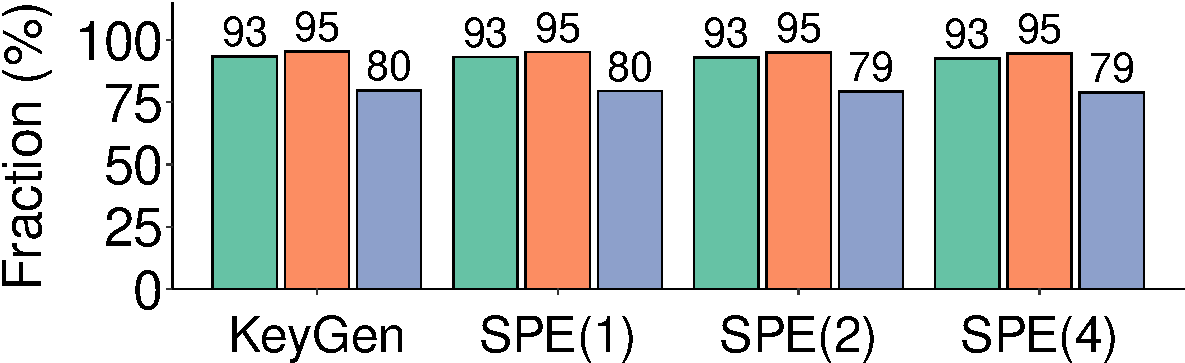
\includegraphics[width=0.33\textwidth]{pic/featurespy/plot/detection/syn/syn-p1-q4-detect.pdf} &
        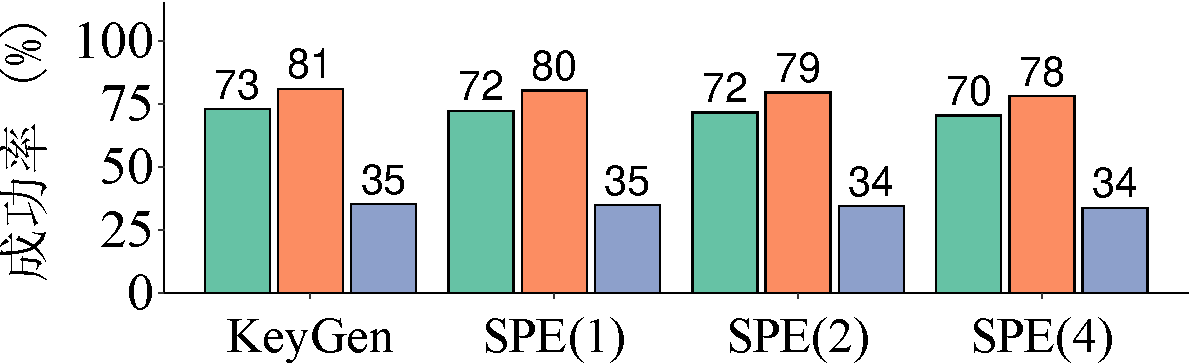
\includegraphics[width=0.33\textwidth]{pic/featurespy/plot/detection/syn/syn-p4-q16-detect.pdf} &
        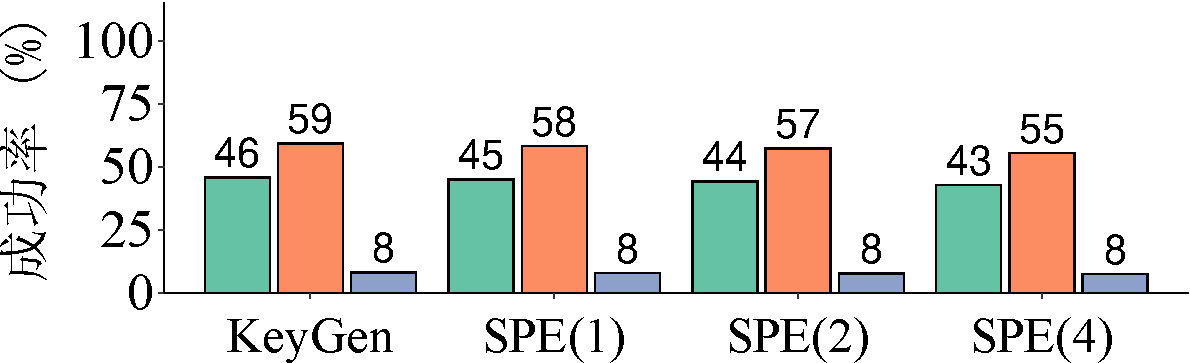
\includegraphics[width=0.33\textwidth]{pic/featurespy/plot/detection/syn/syn-p8-q32-detect.pdf}\\
        \mbox{\small (a) $\textrm{SYNChunk}(1, 4)$}&
        \mbox{\small (b) $\textrm{SYNChunk}(4, 16)$}&
        \mbox{\small (c) $\textrm{SYNChunk}(8, 32)$}\\
    \end{tabular}
    \vspace{-6pt}
    \caption{(Exp\#2) Similarity detection on ciphertext chunks. We evaluate the fraction of similar chunks that are assigned with the same feature key (for KeyGen), as well as that can be detected by examining similarity indicators (for each SPE$(i)$ that configures the first $i$ data blocks of each plaintext chunk as the corresponding similarity indicator).}
    \vspace{-6pt}
    \label{fig:expDetectionSynDetect}
\end{figure*}

Figure~\ref{fig:expDetectionSynDetect} collectively presents the results for the synthetic datasets that have small (SYNChunk$(1, 4)$), medium (SYNChunk$(4, 16)$) and large (SYNChunk$(8, 32)$) modifications among similar chunks, respectively. Compared to {\tt allFeature}, the instances {\tt firstFeature} and {\tt minFeature} generate identical feature keys for more similar chunks, especially when the modifications are large (e.g., 45.7\% for {\tt firstFeature} and 59.3\% for {\tt minFeature} vs. 8.1\% for {\tt allFeature}).
Also, {\tt minFeature} outperforms {\tt firstFeature}, possibly due to the fact that the minimum content feature is more robust against random changes on chunk contents. In addition, we observe that SPE preserves similarity after encryption. Specifically, by examining the similarity indicators in ciphertext chunks, we detect up to 95.2\%, 80.2\% and 58.3\% similar chunks in SYNChunk$(1, 4)$, SYNChunk$(4, 16)$ and SYNChunk$(8, 32)$, respectively.


% For example, in SYNChunk$(8, 32)$, both instances assign a half (e.g., ) of similar chunks with the same feature key, while {\tt allFeature} only generates an identical key for 8.1\% similar chunks.



% \paragraph{Exp\#3 (Similarity detection on ciphertext chunks in real-world workloads).}
% We build on Linux and CouchDB to study the similarity detection of \sysnameF in real-world workloads. Informed by Exp\#1, we consider three similarity measurements that two plaintext chunks are similar if they have one (low similarity), two (medium similarity), and three (high similarity) identical features, respectively. We aim to detect the pairs of similar plaintext chunks based on the corresponding ciphertext chunks that are processed in a batch of a window of chunks. We evaluate the {\em detection coverage} as the ratio of the number of similar chunk pairs that are successfully detected over that in entirety in each window. Here, we focus on {\tt fistFeature} and {\tt minFeature}, since {\tt allFeature}  only detects a small fraction of similar chunks (Exp\#2), and consider each instance FeatureSpy$(i)$, which builds on SPE$(i)$ to configure the first $i$ blocks of each plaintext chunk as the corresponding indicator.

% \begin{figure}[t]
%     \centering
%     
\includegraphics[height=0.1in]{pic/featurespy/plot/detection/real/realBarPlot_legend.pdf}\\
%     \begin{tabular}{cc}
%       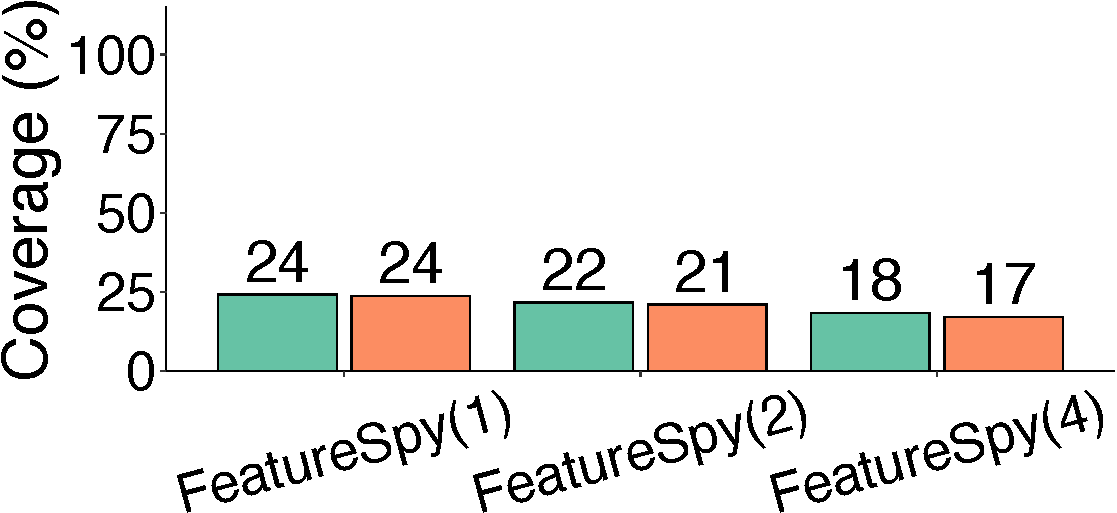
\includegraphics[width=0.23\textwidth]{pic/featurespy/plot/detection/real/linux-5K-1F.pdf} &
%       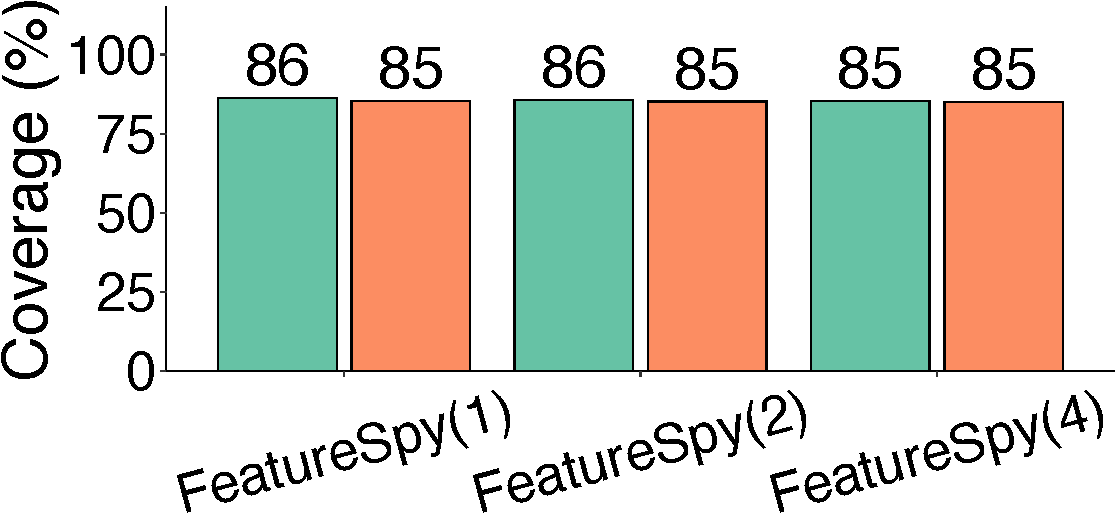
\includegraphics[width=0.23\textwidth]{pic/featurespy/plot/detection/real/couch-5K-1F.pdf} \\
%       \multicolumn{1}{c}{\small (a) One common feature (Linux)} & \multicolumn{1}{c}{\small (b) One common feature (CouchDB)} \\
%       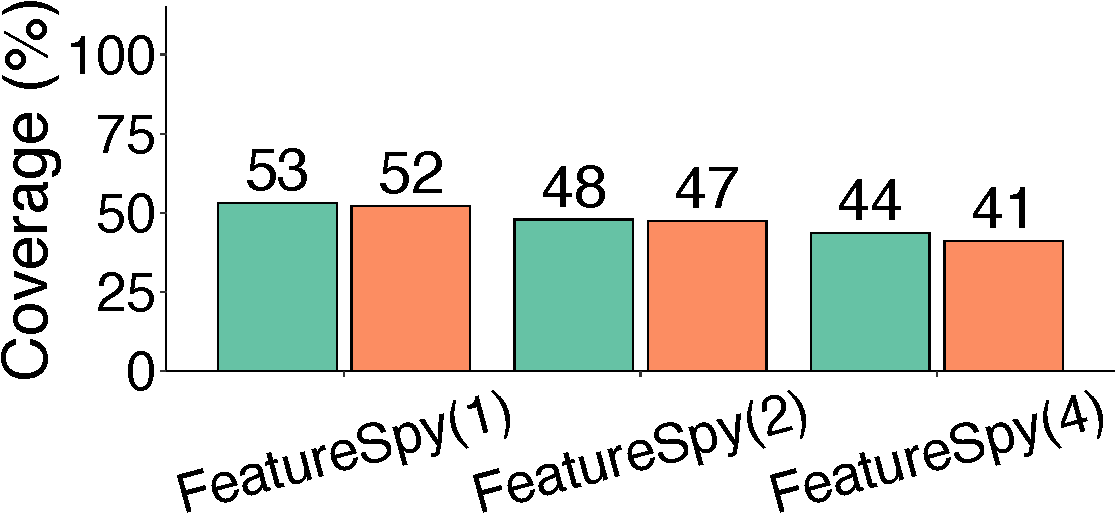
\includegraphics[width=0.23\textwidth]{pic/featurespy/plot/detection/real/linux-5K-2F.pdf} &
%                                                                                     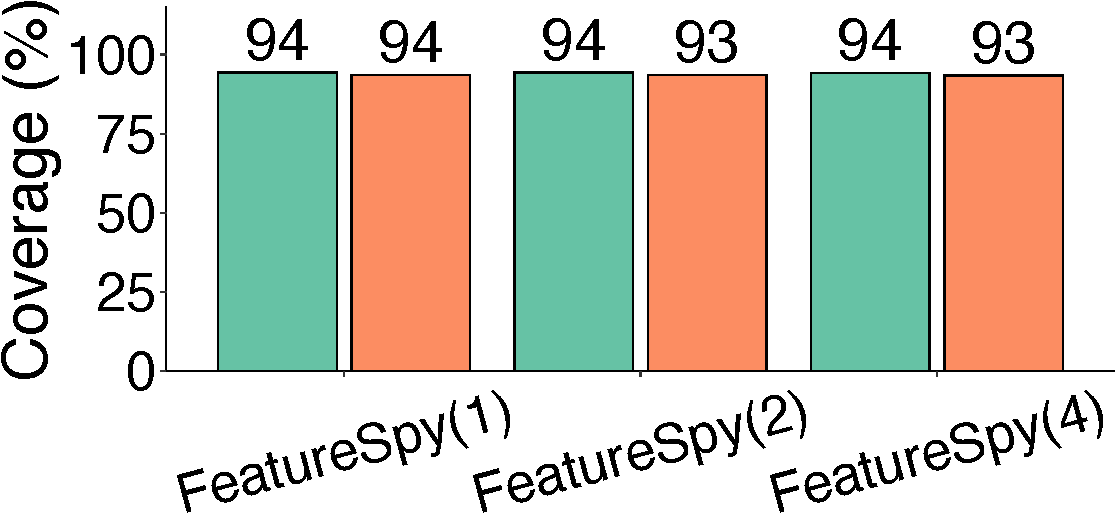
\includegraphics[width=0.23\textwidth]{pic/featurespy/plot/detection/real/couch-5K-2F.pdf} \\
%             \multicolumn{1}{c}{\small (a) One common feature in Linux} & \multicolumn{1}{c}{\small (b) One common feature in CouchDB} \\

%       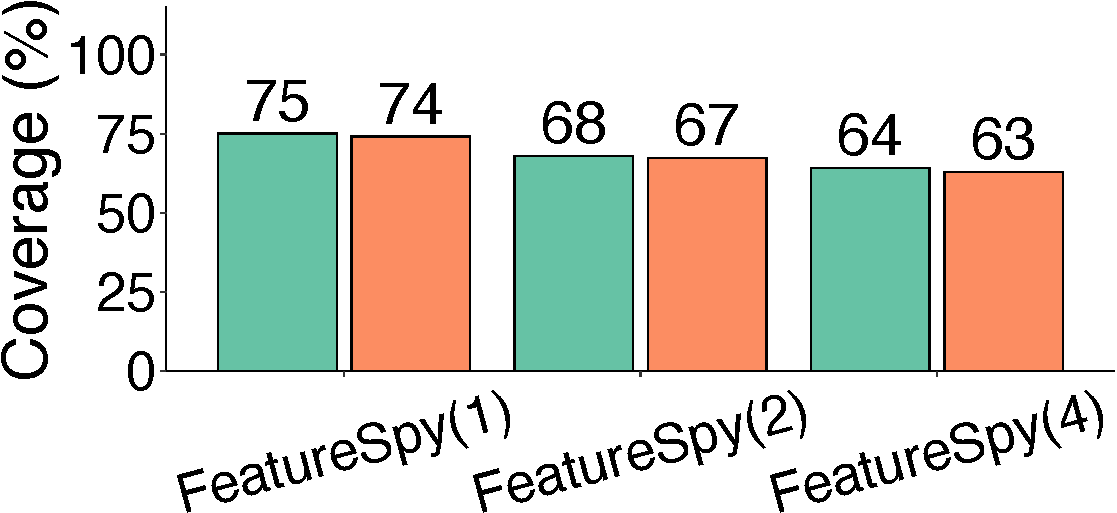
\includegraphics[width=0.23\textwidth]{pic/featurespy/plot/detection/real/linux-5K-3F.pdf} &
%                                                                                     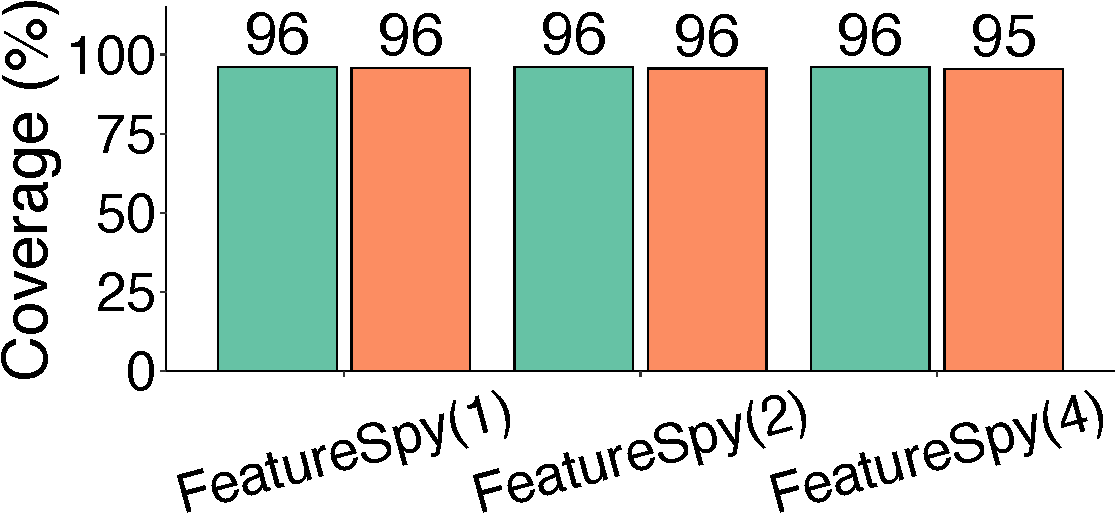
\includegraphics[width=0.23\textwidth]{pic/featurespy/plot/detection/real/couch-5K-3F.pdf} \\
%                   \multicolumn{1}{c}{\small (a) One common feature in Linux} & \multicolumn{1}{c}{\small (b) One common feature in CouchDB} \\

%     \end{tabular}
%     \vspace{-5pt}
%     \caption{(Exp\#3) Similarity detection on ciphertext chunks in real-world workloads. FeatureSpy$(i)$ denotes the instance that uses SPE$(i)$ as the underlying primitive.}
%     \vspace{-5pt}
%     \label{fig:expDetectionReal}
% \end{figure}

% Figure~\ref{fig:expDetectionReal} presents the average results (from all available windows) when we fix the window size at 5\,K chunks. In general, a relaxed similarity measurement leads to a low detection coverage, since each window includes many similar chunks that have significantly distinct contents under the relaxed measurement. For example, when we increase the number of common features (to measure similarity) from one to three, the detection coverage in Linux increases from about 24\% to up to 75\% (in FeatureSpy(1)). The similarity measurement does not affect CouchDB too much, since it only has a few similar chunk pairs (e.g., 6.3 in CouchDB vs. 155.9 in Linux measured by a single common feature) in each window.




% the average number of similar chunk pairs reduces from 155.9 to 10.4 in each Linux window, and.

% Recall from \S\ref{sub:attack}, we consider that chunks modified in a small range are similar (that is, our detection goal is to find chunks with minor modification in a small range). We perform random modifications based on an 8 KiB random chunk to analyze the effectiveness of feature-based similarity detection. Specifically, we first generate an 8 KiB random chunk as base chunk $M$, and then randomly select $p=1 \sim 4$ locations with $q=1 \sim 4$ bytes at each location to modify the chunk $M$ to generate a similar chunk $M'$. Note that, for each $(p,q)$ configuration, we generate $10K$ distinct similar chunks $\{M'\}$. We calculate the frequency of at most $i (i=1,2,3,4)$ features in the set of similar chunks $\{M'\}$ that is the same as the original chunk $M$ as the effectiveness of similarity detection based on feature extraction.

% Figure~\ref{fig:expDetectionSynSim} shows the result, in the case of $p=2,4$ and $q=1,2,4$. As the modification position increases, the probability that multiple features match is significantly reduced. For example, when $p=4$, the probability that all 4 features are matching is only about $40\%$, which is about $2/3$ of that when $p=2$. But the impact of increasing modified bytes number is relatively small. For example, when $p=4$, the change of $q$ from 1 to 4 only reduces the effectiveness of the similarity check based on 4 features from $42.19\%$ to $41.32\%$. At the same time, the effectiveness of the similarity check based on 1 feature is maintained at a level close to $100\%$, and it is minimally affected by the modification position and bytes number. Based on this observation, we decided to use any 1 feature that is the same as the basis for subsequent experiments to determine whether the chunks are similar.


% pic/featurespy/plot each (p,q): 1-2-3-4 feature match ratio + min-first-all feature match + prefix L=1-16-32 block match under min-first-all feature key.





% \begin{figure}[t]
%     \centering
%     \includegraphics[height=0.1in]{pic/featurespy/plot/detection/real/realBarPlotSimilar_legend.pdf}\\
%     \begin{tabular}{@{\ }c@{\ }c}
%         \includegraphics[width=0.23\textwidth]{pic/featurespy/plot/detection/real/similarChunkCouch.pdf} &
%         \includegraphics[width=0.23\textwidth]{pic/featurespy/plot/detection/real/similarChunkLinux.pdf}\\
%         \mbox{\makecell[c]{\small (a) CouchDB}}&
%         \mbox{\makecell[c]{\small (b) Linux Kernel}}\\
%     \end{tabular}
%     \vspace{-5pt}
%     \caption{(Exp\#3) Average number of similar chunks per window under three different window size (1K,5K, and 10K).}
%     \vspace{-5pt}
%     \label{fig:expDetectionRealSimilarChuks}
% \end{figure}

% 2 figures : couchdb + linux
% 1 feature match: min-first-all feature match + false positive + prefix L=1-16-32 block match under min-first-all feature key + false positive.

% We also analyze the effectiveness of \sysnameF based on real-world datasets. Here we use {\em CouchDB Docker image} and {\em Linux Kernel source code} datasets which contains original content. After chunking the original content into chunks with an average size of 8 KiB, we group the chunks into similar groups based on each distinct feature. Subsequently, we calculate the probability that the chunks in each similar group will generate the same key under the three key generation mechanisms and the probability of generating the same indicator as the effectiveness of \sysnameF. According to Figure~\ref{fig:expDetectionReal}, we found that unlike in the case of random data, the effect of first-feature-based key generation is better than that of the min-feature-based scheme, and the similarity check ability for the indicators decreases more than that in synthetic data when increasing the indicator length. We believe that is because the similarity of the chunks in the real-world dataset is far inferior to the similarity between the generated similar chunks. This led us to decide to use $L=2$ blocks as the indicator length for attack detection in \sysnameF. By using this length, we can achieve effective detection of attack behavior (generating a large number of very similar chunks) while reducing the information leakage of indicators.
% {\em Limitations}. We have not analyzed the false-positive of the schemes here. This is because we are unable to define the degree of similarity of the chunks, which makes us unable to delineate the scope of the false-positive. And it does not affect the detection of the {\em Learning-content Attack}. This will be our feature work.

\paragraph{Exp\#3 (Case study of attack detection).}
We expand the case study in \S\ref{sub:attack} to study how \sysnameF detects the learning-content attack of inferring salaries and sign-on bonuses.
We configure \sysnameF with a fixed ratio threshold $T$ = 3\% and a similarity indicator that has a size of two blocks (or equivalently 32 bytes).
Recall from \S\ref{sub:attack} that the adversary needs to fake 101 $\times$ 31 = 3131 adversarial offers, where the annual salary and the sign-on bonus have 101 and 31 possible values, respectively. To simulate the adversary that uploads adversarial offers in ordinary snapshots (otherwise it can be  detected more easily), we randomly insert all adversarial offers into each Linux/CouchDB snapshot, perform chunking on each individual file of the {\em attack snapshot} (that includes adversarial offers) as existing chunk-based deduplication approaches \cite{fsl, meyer11}, and further apply SPE on the chunks. We evaluate the {\em detection rate}, which is the ratio of the number of such attack snapshots that \sysnameF successfully detects by the total number of attack snapshots. Also, we let \sysnameF process each raw snapshot (without adversarial injections), and evaluate the {\em false rate}, which is the ratio of the number of snapshots that \sysnameF misjudges by the total number of raw snapshots. We show how \sysnameF detects the learning-content attack, followed by the overall detection results.
Here, we do not consider FSL and MS for evaluation, since they have no actual data contents.

\begin{figure*}[t]
    \centering
    
\includegraphics[width=0.5\textwidth]{pic/featurespy/plot/detection/overall/prefixDistribution_legend.pdf}\\
    \begin{tabular}{@{\ }c@{\ }c@{\ }c}
        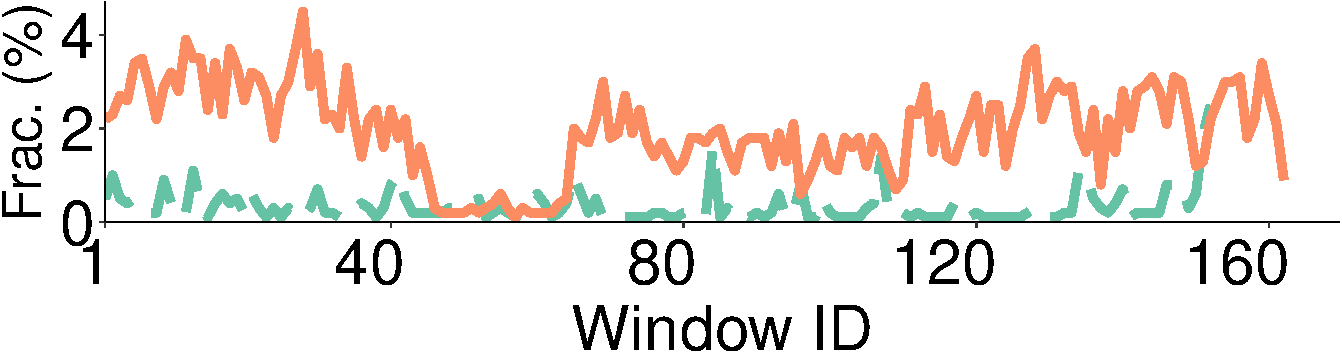
\includegraphics[width=0.33\textwidth]{pic/featurespy/plot/detection/overall/prefixDistribution-1000-Linux-first.pdf} &
        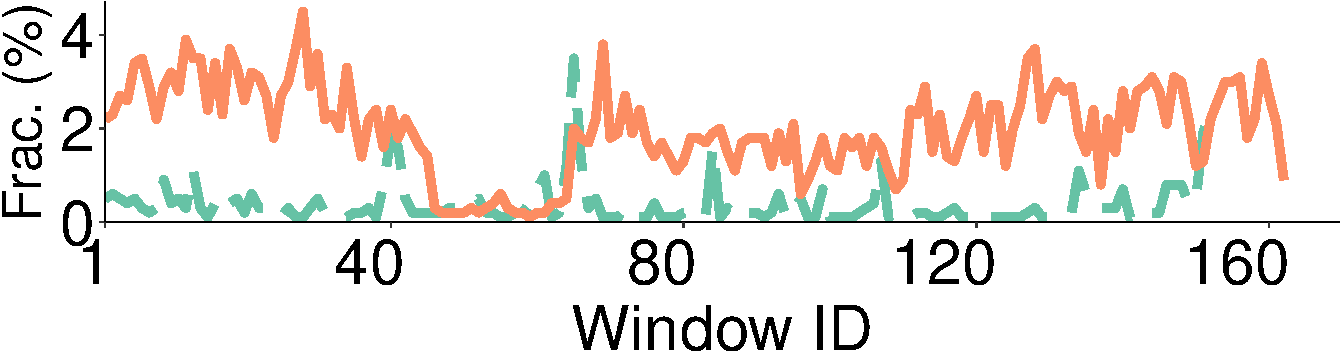
\includegraphics[width=0.33\textwidth]{pic/featurespy/plot/detection/overall/prefixDistribution-1000-Linux-min.pdf} &
        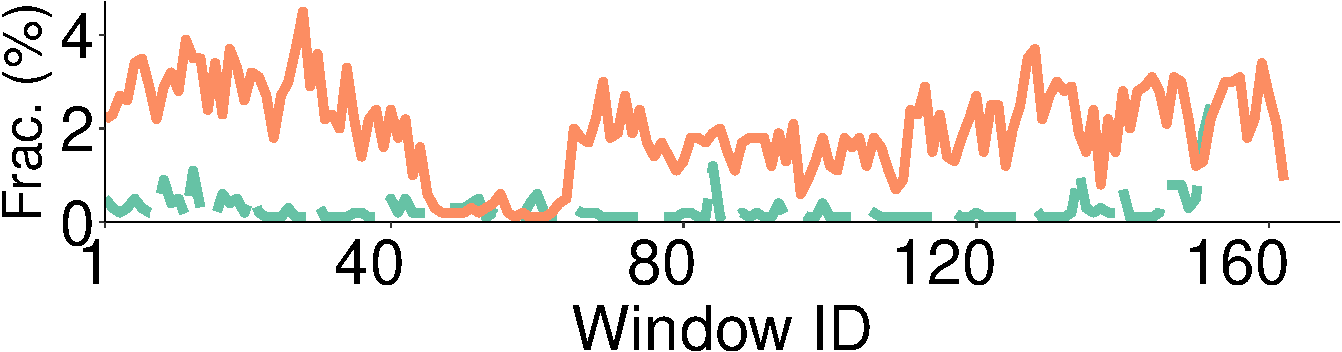
\includegraphics[width=0.33\textwidth]{pic/featurespy/plot/detection/overall/prefixDistribution-1000-Linux-all.pdf} \\
        \mbox{\makecell[c]{\small (a) {\tt firstFeature}}}&
        \mbox{\makecell[c]{\small (b) {\tt minFeature}}}&
        \mbox{\makecell[c]{\small (c) {\tt allFeature}}}\\
    \end{tabular}
    \vspace{-5pt}
    \caption{(Exp\#3) An attack detection example to show that {\tt firstFeature}, {\tt minFeature} and {\tt allFeature} process the same Linux snapshot that are with (i.e., attack) and without (i.e., raw) adversarial injections. We present the fraction of the most number of chunks that have an identical similarity indicator over the total number of chunks (fixed at $W$ = 1\,K) in each window. }
    \label{fig:expDetectionOverall}
  \end{figure*}

Figure~\ref{fig:expDetectionOverall} compares \sysnameF instances in detecting the learning-content attack in the same Linux snapshots (i.e., v5.13) that are injected with (i.e., attack) or without (i.e., raw) adversarial offers. Specifically, the x-axis indexes the processing window (whose size is fixed at 1\,K here), while the y-axis shows the fraction of the {\em most} number of ciphertext chunks that have the same similarity indicator over the total number of all chunks (i.e., 1\,K) in the corresponding window. We observe that all three instances can effectively detect the learning-content attack, since they have {\em at least} one window in the attack snapshot, such that the fraction of the ciphertext chunks that have the same similarity indicator  is greater than $T$ (i.e., 3\%). On the other hand, {\tt minFeature} suffers from a {\em false positive}, since it even has a normal window (e.g., the 65-th window in raw), in which the fraction (e.g., 3.5\%) of the chunks that are detected similar is greater than $T$.

\begin{figure}[t]
    \centering
    
\includegraphics[width=0.25\textwidth]{pic/featurespy/plot/detection/overall/effectiveness-falsePositive_legend.pdf}
    \vspace{5pt}\\
    \begin{tabular}{@{\ }c@{\ }c}
        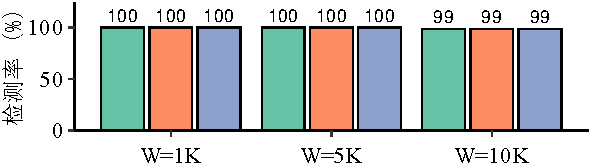
\includegraphics[width=0.286\textwidth]{pic/featurespy/plot/detection/overall/effectivenessLinux.pdf} &
        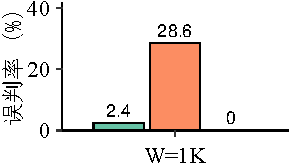
\includegraphics[width=0.16\textwidth]{pic/featurespy/plot/detection/overall/falsePositiveLinux.pdf}\\
        \mbox{\small (a) Detection rate} &
        \mbox{\small (b) False rate}\\
    \end{tabular}
    \vspace{-6pt}
    \caption{(Exp\#3) Overall detection and false rates in each Linux snapshot. Note that {\tt allFeature} does not have any false positives.}
    \vspace{-6pt}
    \label{fig:expDetectionOverallFalsePositive}
\end{figure}


Figure~\ref{fig:expDetectionOverallFalsePositive} presents the overall detection and false rates in Linux when we configure the window sizes at 1\,K, 5\,K, and 10\,K, respectively. In general, \sysnameF achieves a high detection rate (e.g., at least 98.6\%) in Linux snapshots. However, a large window slightly degrades the detection rate, since a relatively small fraction of ciphertext chunks have an identical similarity indicator.
In addition, \sysnameF incurs false positives only when the window size is 1\,K (Figure~\ref{fig:featureDistribution}(b)), since the raw snapshots originally have significant fractions of similar chunks. Even in this case, {\tt allFeature} does not have any false positive, since it only detects a small number of similar chunks. On the other hand, {\tt minFeature} that detects more similar chunks (Exp\#2) incurs 28.6\% false positives.

%Furthermore, {\tt minFeature} incurs more false positives (e.g., 28.6\%) than the other two instances, since it can detect more similar chunks (Exp\#2).

In addition to Linux, we evaluate \sysnameF in CouchDB and find that all \sysnameF instances successfully detect the learning-content attack in all CouchDB snapshots (i.e., 100\% of detection rate)  without introducing any false positives. The possible reason is that each CouchDB snapshot has many unsimilar chunks and \sysnameF can immediately detect the distribution changes (of similar chunks) when many adversarial similar chunks are injected.

%a small size (e.g., 282.5\,MiB on average), and it is insufficient to obfuscate the distribution of the similar chunks in the faked offers.



% We use the latest and oldest versions of both Linux (v2.6.11 and v5.13) and CouchDB (v2.5.2 and v6.6.2) datasets as raw backup streams, which \sysnameF will store each file in each stream in turn. At the same time, We consider that the attacker randomly inserts the faked offer files into the raw backup stream to launch the attack and try to escape \sysnameF's detection. Then, we analyze the top frequency of indicators in each window under different window sizes to verify whether \sysnameF can distinguish mixed fake file stream from the raw backup stream. Here, we use the min-feature-based key generation scheme along with indicator length $L=2$ blocks as our default configuration of \sysnameF.

% Figure~\ref{fig:expDetectionOverall} shows the most frequently indicator's frequency in each window of both raw backup stream and mixed fake file stream. Note that, in some cases, the window number of mixed fake file streams is more than the raw backup stream due to the added chunks. In all cases, the mixed fake file stram has the highest frequency in some windows which is higher than the highest frequency in all windows of the raw backup stream. This allows us to set an appropriate threshold $T$ according to the window size to stop the attacker's potential offensive behavior. For example, when the window size is 1K, we could set threshold $T = 0.03$ to detect malicious behavior.

\paragraph{Exp\#4 (Impact of different target files).}
We now study the effectiveness of \sysnameF when it is used to detect the learning-content attack against each synthetic file SYNFile$(x, y)$ (recall that $x$ is the number of unknown variables in the file, and $y$ is the number of possible values for each variable). To attack SYNFile$(x, y)$, we enumerate $x \times y$ adversarial files, randomly insert them into the last Linux snapshot (that has the maximum size of 985.9\,MiB among other snapshots), and evaluate the detection rate of \sysnameF  (configured with a fixed $T$ = 3\%) over 100 runs.



% attack detection. We focus on each synthetic file
% use the synthetic dataset SYNFile$(x, y)$ to explore the impact of various parameter changes in the attack detection. Specifically, we first randomly generate a 4\,KiB base file, and then select $x=3,6,9$ variables among the file for random modification. The message space of each variable is $y=2^{9},2^{10},2^{11}$. In this way, we get the files in the dataset SYNFile$(x, y)$ which will be used for the attack. The file number is $x\times y$ (for example, if the random variable $x=3$ and the message space are $2^{10}$, the total number of files is $3072$). We insert SYNFile$(x, y)$ into the last snapshot of the Linux dataset as in Exp\#3, and then check the detection of \sysnameF under different parameters through 100 random tests.

\begin{figure}[t]
    \centering
    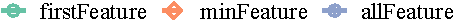
\includegraphics[width=0.25\textwidth]{pic/featurespy/plot/detection/trade-off/trade_off_legend.pdf}
    \vspace{5pt}\\
    \begin{tabular}{@{\ }c@{\ }c@{\ }c}
        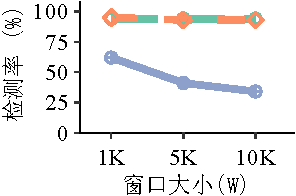
\includegraphics[width=0.15\textwidth]{pic/featurespy/plot/detection/trade-off/varyWindow_linux.pdf} &
        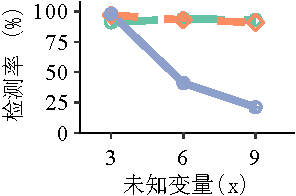
\includegraphics[width=0.15\textwidth]{pic/featurespy/plot/detection/trade-off/varyModifyPos_linux.pdf}&
        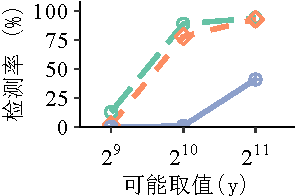
\includegraphics[width=0.15\textwidth]{pic/featurespy/plot/detection/trade-off/varyFileNumber_linux.pdf} \\
        \makecell[c]{\small (a) Vary $W$ \\ \small against SYNFile$(6, 2048)$} &
        \makecell[c]{\small (b) Fix W = 5\,K \\ \small against SYNFile$(\cdot, 2048)$} &
        \makecell[c]{\small (c) Fix W = 5\,K \\ \small against SYNFile$(6, \cdot)$} \\
    \end{tabular}
    \vspace{-6pt}
    \caption{(Exp\#4) Impact of different target files.}
    \vspace{-6pt}
    \label{fig:expDetectionTradeOff}
\end{figure}

Figure~\ref{fig:expDetectionTradeOff}(a) presents the results when we vary the window size $W$ to attack SYNFile$(6, 2048)$. The detection rates of {\tt firstFeature} and {\tt minFeature} are robust against the increase of $W$ (e.g., always stay above 93\%), but that of {\tt allFeature} drops to 34\%. The reason is that {\tt allFeature} can only detect a small number of similar chunks (Exp\#2), which take a low fraction when $W$ is large. Figure~\ref{fig:expDetectionTradeOff}(b) presents the results when we vary the number of unknown variables $x$ in the target file. We observe that the detection rate of {\tt allFeature} again drops dramatically to 21\% when $x$ = 9, since it fails to detect the similar chunks that have more different regions.


Figure~\ref{fig:expDetectionTradeOff}(c) presents the results when we vary the number $y$ of possible values for each variable in the target file. All three instances achieve a low detection rate (e.g., up to 13\%) when $y$ is 512. The reason is that the target file has a low entropy, and the adversary only needs to construct a small number of similar contents.  \sysnameF is ineffective to detect the learning-content attack in this case.
One possible solution is to configure a small $T$ or $W$ to report an attack case when a few similar chunks are detected, yet it increases the possibility of misjudgements in different workloads.
We pose a future work for how to automatically balance the trade-off between detecting attack on low-entropy files and minimizing misjudgements when working on different workloads.



%has the highest detection rate  (98\%) when $x$ = 3, since the chunks in faked files now have high similarity and {\tt minFeature}
% gives the effect of different window sizes on the three schemes under SYNFile$(6,2^{11})$. It is obvious that with the increase of window size, the detection of minFeature and firstFeature schemes are maintained at a high level (not lower than $93\%$), but the detection of allFeature schemes decreases with the increase of window size. This is because allFeature has the lowest ability to find similar chunks (refer to Exp\#1,\#2), and a larger window size will not significantly increase the number of similar chunks that can be found.

% Figure~\ref{fig:expDetectionTradeOff}(b) shows the result of the fixed window size at $W=5K$, and the message space of each random variable at $y=2^{11}$, then varying the number of random variables $x$. As the number of random variables increases, the detection of minFeature and firstFeature schemes decrease/increase slightly (from $97\%$ to $91\%$ and $91\%$ to $93$, respectively). However, the detection of the allFeature scheme has dropped significantly. This is due to the poor ability of allFeaure scheme to check chunks with low similarity, which coincides with the result of Exp\#2.
% Figure~\ref{fig:expDetectionTradeOff}(c) is the result of fixing the number of random variables $x=6$, and the window size $W=5K$, changing the message space of each random variable. With the increase of the message space, the detection of the three schemes has been significantly improved. This is because the increase of the message space will directly lead to an increase in the number of files in SYNFile$(x, y)$, which will generate a large number of similar chunks. The allFeature scheme finally reaches $41\%$, while the minFeature and firstFeature schemes finally reach $93\%$ and $94\%$. Combining with Exp\#3, we believe that the minFeature scheme has a higher detection but also brings a lot of false positives. The allFeature scheme has no false positives but the detection is low. However, the firstFeature scheme achieves both low false-positive and high detection.